\documentclass[runningheads]{../../../llncs}
\usepackage[paperheight=295mm,paperwidth=210mm]{geometry}
\usepackage{graphicx}
\usepackage{import}
\usepackage{kotex}
\usepackage[dvipsnames]{xcolor}
\usepackage{fancyvrb}
\usepackage{listings}
\usepackage{indentfirst}
\usepackage{tabularx}
\usepackage{underscore}
\usepackage{multicol}
\usepackage{enumitem}
\usepackage{menukeys}
\usepackage{amsmath}
\usepackage{clrscode3e} % https://www.ctan.org/pkg/clrscode3e?lang=en
\usepackage[numbers,square,super]{natbib}
\usepackage{inconsolata} % Inconsolata
\usepackage{mathptmx} % Times New Roman
\usepackage{minted}
\graphicspath{ {./images/} }
\lstset{basicstyle=\footnotesize\ttfamily,breaklines=true}
\renewcommand{\bibname}{참고문헌}
\setlength{\parindent}{1em}
\setlength{\parskip}{1em}
\linespread{1.2}
{\renewcommand{\arraystretch}{1.5}%
\setlength{\tabcolsep}{0.5em}%
\newenvironment{Figure}
  {\par\medskip\noindent\minipage{\linewidth}}
  {\endminipage\par\medskip}
\newcommand{\translation}[1]{\textsuperscript{#1}}
\newlist{algorithm}{enumerate}{10}
\setlist[algorithm]{label*=\arabic*.}
\setlist[algorithm,1]{label=\textbf{\arabic*}}
\setlist[algorithm,2]{label=\textbf{\alph*}}
\setlist[algorithm,3]{label=\textbf{\roman*}}
\setlist[algorithm,4]{label=(\arabic*)}
\setlist[algorithm,5]{label=(\alph*)}
\setlist[algorithm,6]{label=(\roman*)}
\makeatletter
\renewcommand\NAT@citesuper[3]{\ifNAT@swa
\if*#2*\else#2\NAT@spacechar\fi
\unskip\kern\p@\textsuperscript{\NAT@@open#1\if*#3*\else,\NAT@spacechar#3\fi\NAT@@close}%
   \else #1\fi\endgroup}
\makeatother
	
\begin{document}

\title{CSE3013 (컴퓨터공학 설계 및 실험 I) \space \newline PRJ-1 테트리스 프로젝트 1주차 결과 보고서}
\author{서강대학교 컴퓨터공학과 박수현 (20181634)}
\institute{서강대학교 컴퓨터공학과}
\maketitle

\section{목적}
1주차 구현 내용과 작성했던 의사 코드와 실제로 어떻게 다른지 기술하고 복잡도를 보인다. 1주차 과제 내용에 대한 의사 코드와 복잡도를 보인다. 

\section{의사 코드 비교}
의사 코드를 그대로 C 코드로 변환했으며, 실제 코드는 의사 코드와 거의 차이가 없었다. 아래는 의사 코드와 실제 코드의 비교이다.

\subsubsection{\proc{CheckToMove}}: 명령에 따라 블럭을 이동할 수 있는지 판단한다.
블럭 배열 크기인 4개의 행과 4개의 열마다 $\mathcal{O}\left(1\right)$의 작업을 수행하므로, 시간 복잡도는 $\mathcal{O}\left(1\right)$이다.

\begin{codebox}
\Procname{$\proc{CheckToMove}(f, \id{currentBlock}, \id{blockRotate}, \id{blockY}, \id{blockX})$}
\li \For $i \gets 0$ \To $3$
\li \Do
        \For $j \gets 0$ \To $3$
\li     \Do
            \If $\id{block}[\id{currentBlock}][\id{blockRotate}][i][j] \isequal 1$
\li         \Then
                $x \gets \id{blockX} + j$
\li             $y \gets \id{blockY} + i$
\li             \If $\left( 0 \leq x < \id{WIDTH} \mbox{ and } 0 \leq y < \id{HEIGHT} \right) \neq \const{true}$
\li                 \Then \Return $\const{false}$
                \End
\li             \If $f[y][x] \isequal 1$
\li                 \Then \Return $\const{false}$
                \End
            \End
        \End
    \End
\li \Return $\const{true}$
\end{codebox}

\inputminted[xleftmargin=\parindent,linenos,firstline=246,lastline=261]{c}{inc-sources/tetris-week09-experiment.c}

\subsubsection{\proc{DrawChange}}: 명령에 의해 바뀐 부분만 필드에 업데이트한다.
\proc{DrawField}에 $\mathcal{O}\left(\id{WIDTH}\times\id{HEIGHT}\right)$만큼, \proc{DrawBlock}에 $\mathcal{O}\left(1\right)$만큼의
시간이 걸리므로 이 함수의 시간 복잡도는 $\mathcal{O}\left(\id{WIDTH}\times\id{HEIGHT}\right)$이다.

\begin{codebox}
\Procname{$\proc{DrawChange}(f, \id{command}, \id{currentBlock}, \id{blockRotate}, \id{blockY}, \id{blockX})$}
\li \Comment Erase current block
\li $\proc{DrawField}()$
\li \Comment Draw new block
\li $\proc{DrawBlock}(blockY, blockX, currentBlock, blockRotate, \mbox{` '})$
\end{codebox}

\inputminted[xleftmargin=\parindent,linenos,firstline=263,lastline=267]{c}{inc-sources/tetris-week09-experiment.c}

\newpage

\subsubsection{\proc{BlockDown}}: 블럭을 아래로 내린다. 더 이상 내릴 수 없을 경우 현재 블럭을 필드에 고정시키고 다음 블럭을 사용한다. 시간 복잡도는
\proc{CheckToMove}와 \proc{AddBlockToField}에 각각 $\mathcal{O}\left(1\right)$,
\proc{DrawChange}와 \proc{DeleteLine}과 \proc{DrawField}에 각각 $\mathcal{O}\left(\id{WIDTH}\times\id{HEIGHT}\right)$이
걸리므로 $\mathcal{O}\left(\id{WIDTH}\times\id{HEIGHT}\right)$이다.

\begin{codebox}
\Procname{$\proc{BlockDown}(\id{sig})$}
\li \If $\proc{CheckToMove}(f, \id{currentBlock}, \id{blockRotate}, \id{blockY} + 1, \id{blockX})$
\li \Then
        $\id{blockY} = \id{blockY} + 1$
\li     $\proc{DrawChange}(f, \id{command}, \id{currentBlock}, \id{blockRotate}, \id{blockY}, \id{blockX})$
\li \Else
\li     \If $\id{blockY} \isequal 1$
\li     \Then
            $\id{gameOver} \gets \const{true}$
\li     \Else
\li         $\proc{AddBlockToField}(f, \id{currentBlock}, \id{blockRotate}, \id{blockY}, \id{blockX})$
\li         $\id{score} \gets \id{score} + \proc{DeleteLine}(f)$
\li         \Comment Generate new block
\li         $\id{nextBlock}[0] \gets \id{nextBlock}[1]$
\li         $\id{nextBlock}[1] \gets (\mbox{Random integer in 0 .. 6})$
\li         $\proc{DrawNextBlock}(\id{nextBlock})$
\li         $\id{blockY} \gets -1$, $\id{blockX} \gets (\mbox{Center of field})$
\li         $\proc{DrawField}()$
\li         $\proc{PrintScore}(\id{score})$
        \End
    \End
\end{codebox}

\inputminted[xleftmargin=\parindent,linenos,firstline=269,lastline=290]{c}{inc-sources/tetris-week09-experiment.c}

의사 코드에서 $nextBlock[1] \gets (\mbox{Random integer in 0 .. 6})$이 \mintinline[breaklines]{c}{nextBlock[1] = rand() % 7}로,
$blockX \gets (\mbox{Center of field})$이 \mintinline[breaklines]{c}{blockX = WIDTH / 2 - 2}로 구현되었다.

\subsubsection{\proc{AddBlockToField}}: 필드의 주어진 좌표에 현재 블럭을 고정시킨다.
블럭 배열 크기인 4개의 행과 4개의 열마다 $\mathcal{O}\left(1\right)$의 작업을 수행하므로, 시간 복잡도는 $\mathcal{O}\left(1\right)$이다.

\begin{codebox}
\Procname{$\proc{AddBlockToField}(f, \id{currentBlock}, \id{blockRotate}, \id{blockY}, \id{blockX})$}
\li \For $i \gets 0$ \To $3$
\li \Do
        \For $j \gets 0$ \To $3$
\li     \Do
            \If $\id{block}[\id{currentBlock}][\id{blockRotate}][i][j] \isequal 1$
\li         \Then
                $f[\id{blockY} + i][\id{blockX} + j] \gets 1$
            \End
        \End
    \End
\li \Return $\const{true}$
\end{codebox}

\inputminted[xleftmargin=\parindent,linenos,firstline=292,lastline=301]{c}{inc-sources/tetris-week09-experiment.c}

\newpage

\subsubsection{\proc{DeleteLine}}: 꽉 찬 줄이 있는지 체크하고, 있을 경우 줄을 지우고 스코어를 증가시킨다. 모든 열마다
모든 칸이 차 있는지 체크하므로 시간 복잡도는 $\mathcal{O}\left(\id{WIDTH}\times\id{HEIGHT}\right)$이다.

\begin{codebox}
\Procname{$\proc{DeleteLine}(f)$}
\li $erased \gets 0$
\li \For $i \gets 0$ \To $\id{HEIGHT} - 1$
\li \Do
        $flag \gets \const{true}$
\li     \For $j \gets 0$ \To $\id{WIDTH} - 1$
\li     \Do
            \If $f[i][j] \isequal 0$
\li         \Then
                $flag \gets \const{false}$
            \End
        \End
\li     \If $flag \isequal \const{true}$
            \Then
\li             $erased \gets erased + 1$
\li             \For $y \gets i$ \Downto $1$
\li             \Do
                    \For $x \gets 0$ \To $\id{WIDTH} - 1$
\li                 \Do
                        $f[y][x] \gets f[y - 1][x]$
                    \End
                \End
\li             \For $x \gets 0$ \To $\id{WIDTH} - 1$
\li             \Do
                    $f[0][x] \gets 0$
                \End
\li             $i \gets i - 1$
            \End
        \End
    \End
\li \Return $100 \times \id{erased}^2$
\end{codebox}

\inputminted[xleftmargin=\parindent,linenos,firstline=303,lastline=326]{c}{inc-sources/tetris-week09-experiment.c}

\section{과제}

프로젝트 요구사항에 추가로 필드가 색상 정보를 담을 수 있도록 자료구조를 다소 수정하였다.
필드 각각의 칸에 담겨 있는 수가 0이면 비어 있음을 뜻하고, 0이 아니면 차 있음을 뜻하며, 0이 아닐 경우 렌더해야 하는 색상을 의미하도록 정의를 바꾸었다.

\begin{multicols}{2}
    \begin{Figure}
		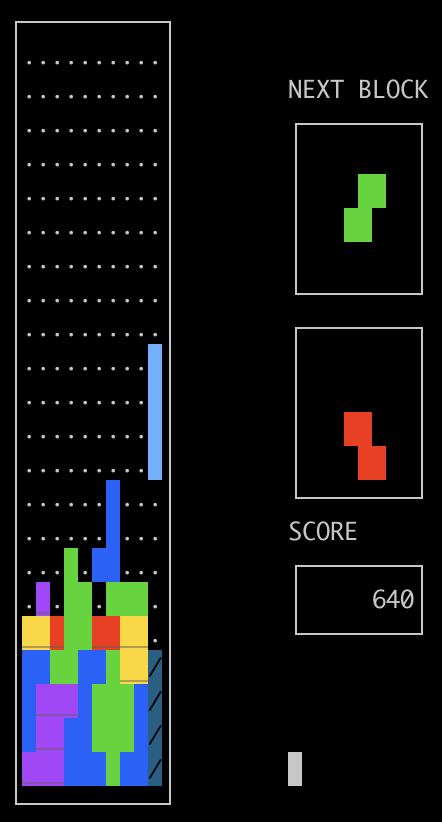
\includegraphics[width=\linewidth]{colors256}
        \label{fig:colors256}
	\end{Figure}
	\columnbreak
    \begin{Figure}
		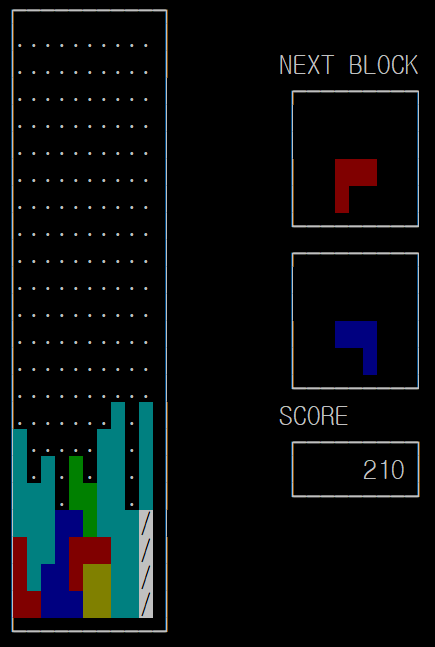
\includegraphics[width=\linewidth]{colors8}
        \label{fig:colors8}
	\end{Figure}
\end{multicols}

256 색상 렌더를 지원하는 터미널에서는 256 색상을 사용해 렌더했고, 그렇지 않은 터미널에서는 8 색상만을 이용해 렌더했다.

\subsection{그림자 렌더}

\subsubsection{\proc{DrawBlock}}: 블럭을 그린다. 시간 복잡도는 $\mathcal{O}\left(1\right)$이다.

\begin{codebox}
\Procname{$\proc{DrawBlock}(y, x, \id{blockID}, \id{blockRotate}, \id{tile}, \id{isShadow})$}
\li \For $i \gets 0$ \To $3$
\li \Do
        \For $j \gets 0$ \To $3$
\li     \Do
            \If $\id{block}[\id{blockID}][\id{blockRotate}][i][j] \isequal 1$ and $i + y \geq 0$
\li         \Then
                Move cursor to $(i + y + 1, \, j + x + 1)$
\li             Print character
            \End
        \End
    \End
\li Move cursor to $(\id{HEIGHT}, \, \id{WIDTH} + 10)$
\end{codebox}

\inputminted[xleftmargin=\parindent,linenos,firstline=190,lastline=210]{c}{inc-sources/tetris-week09-homework.c}

\subsubsection{\proc{GhostY}}: 현재 블럭이 그대로 떨어질 경우 도달하는 블럭의 $y$좌표를 계산한다. 시간 복잡도는 $\mathcal{O}\left(HEIGHT\right)$이다.
\begin{codebox}
\Procname{$\proc{GhostY}(y, x, \id{blockID}, \id{blockRotate})$}
\li \While $\proc{CheckToMove}(\id{field}, \id{nextBlock}[0], \id{blockRotate}, y + 1, x)$
\li \Do
        $y \gets y + 1$
    \End
\li \Return $y$
\end{codebox}

\inputminted[xleftmargin=\parindent,linenos,firstline=292,lastline=295]{c}{inc-sources/tetris-week09-homework.c}

\subsubsection{\proc{DrawShadow}}: 그림자를 그린다. 시간 복잡도는 $\mathcal{O}\left(HEIGHT\right)$이다.

\begin{codebox}
\Procname{$\proc{DrawBlock}(y, x, \id{blockID}, \id{blockRotate}, \id{tile}, \id{isShadow})$}
\li $y \gets \proc{GhostY}(y, x, \id{blockID}, \id{blockRotate})$
\li $\proc{DrawBlock}(y, x, \id{blockID}, \id{blockRotate}, \mbox{`/'}, 1)$
\end{codebox}

\inputminted[xleftmargin=\parindent,linenos,firstline=378,lastline=381]{c}{inc-sources/tetris-week09-homework.c}

\subsubsection{\proc{DrawBlockWithFeatures}}: 블럭과 그림자를 그린다. 시간 복잡도는 $\mathcal{O}\left(HEIGHT\right)$이다.

\begin{codebox}
\Procname{$\proc{DrawBlockWithFeatures}(y, x, \id{blockID}, \id{blockRotate})$}
\li $\proc{DrawShadow}(y, x, \id{blockID}, \id{blockRotate})$
\li $\proc{DrawBlock}(y, x, \id{blockID}, \id{blockRotate}, \mbox{` '}, 0)$
\end{codebox}

\inputminted[xleftmargin=\parindent,linenos,firstline=383,lastline=386]{c}{inc-sources/tetris-week09-homework.c}

\subsection{다음 블록 슬롯 추가}

\texttt{BLOCK_NUM}의 값을 바꿀 경우 칸이 늘어나게 설계하였다. NEXT 슬롯의 높이는 6칸이므로, 원래 SCORE 슬롯이 $Y$ 좌표 10에 그려졌다면
수정된 이후에는 $-2 + 6 \times BLOCK\_NUM$이 된다.

\proc{InitTetris} - 다음 블럭을 초기화하는 부분이 아래와 같이 수정되었다.
\inputminted[xleftmargin=\parindent,linenos,firstline=54,lastline=56]{c}{inc-sources/tetris-week09-homework.c}

\proc{DrawNextBlock} - 다음과 같이 수정되었다. 시간 복잡도는 $\mathcal{O}\left(BLOCK\_NUM\right)$이다.
\inputminted[xleftmargin=\parindent,linenos,firstline=174,lastline=188]{c}{inc-sources/tetris-week09-homework.c}

\proc{BlockDown} - 다음 블럭 목록을 업데이트하는 부분이 아래와 같이 수정되었다.
\inputminted[xleftmargin=\parindent,linenos,firstline=315,lastline=317]{c}{inc-sources/tetris-week09-homework.c}

\subsection{점수 계산 방법 변경}
\proc{AddBlockToField} - 다음과 같이 수정되었다. 시간 복잡도는 $\mathcal{O}\left(1\right)$이다.
\inputminted[xleftmargin=\parindent,linenos,firstline=329,lastline=351]{c}{inc-sources/tetris-week09-homework.c}

\proc{BlockDown} - 점수가 추가되는 부분이 다음과 같이 수정되었다.
\inputminted[xleftmargin=\parindent,linenos,firstline=308,lastline=324]{c}{inc-sources/tetris-week09-homework.c}

\end{document}
